% Source: graduate-coursework/Sp26/CSCE775/course_notes/practice_problems.tex

\documentclass[border=4pt]{standalone}
\usepackage{amsmath, amssymb, amsthm}
\usepackage{tikz}
\usepackage{xcolor}
\usetikzlibrary{arrows.meta, positioning, shapes.geometric}

\definecolor{Garnet}{RGB}{115, 0, 10}
\definecolor{Atlantic}{RGB}{70, 106, 159}
\definecolor{Congaree}{RGB}{31, 65, 77}
\definecolor{NinetyBlack}{RGB}{54, 54, 54}
\definecolor{FiftyBlack}{RGB}{162, 162, 162}

\begin{document}
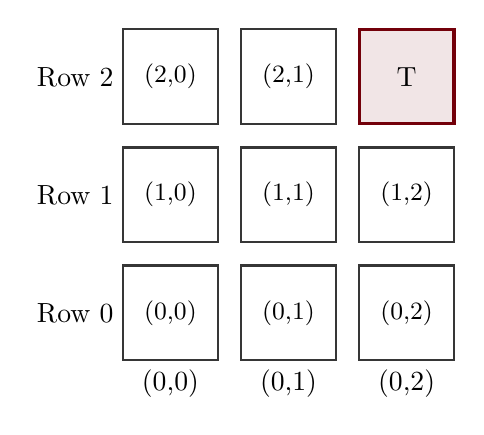
\begin{tikzpicture}[
    cell/.style={rectangle, minimum size=1.2cm, draw=NinetyBlack, thick},
    terminal/.style={rectangle, minimum size=1.2cm, draw=Garnet, very thick, fill=Garnet!10}
]

% Grid cells (row, col) - (0,0) is bottom-left
\foreach \row in {0,1,2} {
    \foreach \col in {0,1,2} {
        \ifnum\row=2
            \ifnum\col=2
                \node[terminal] at (\col*1.5, \row*1.5) {T};
            \else
                \node[cell] at (\col*1.5, \row*1.5) {};
            \fi
        \else
            \node[cell] at (\col*1.5, \row*1.5) {};
        \fi
    }
}

% Labels
\node[below] at (0, -0.6) {(0,0)};
\node[below] at (1.5, -0.6) {(0,1)};
\node[below] at (3, -0.6) {(0,2)};
\node[left] at (-0.6, 0) {Row 0};
\node[left] at (-0.6, 1.5) {Row 1};
\node[left] at (-0.6, 3) {Row 2};

% Coordinate labels
\node[font=\small] at (0, 0) {(0,0)};
\node[font=\small] at (1.5, 0) {(0,1)};
\node[font=\small] at (3, 0) {(0,2)};
\node[font=\small] at (0, 1.5) {(1,0)};
\node[font=\small] at (1.5, 1.5) {(1,1)};
\node[font=\small] at (3, 1.5) {(1,2)};
\node[font=\small] at (0, 3) {(2,0)};
\node[font=\small] at (1.5, 3) {(2,1)};

\end{tikzpicture}
\end{document}
